\documentclass[tikz,border=3pt]{standalone}
\usepackage{times}
\usepackage{amsmath}
\usepackage{tikz}

% Color definitions recovered from Figure 1 in the supplied preprint.
\definecolor{genfill}{HTML}{CBD5E4}
\definecolor{draftfill}{HTML}{F0E2C8}
\definecolor{savedfill}{HTML}{D6EEDA}
\definecolor{draftline}{HTML}{A88046}
\definecolor{savedline}{HTML}{237846}

\begin{document}
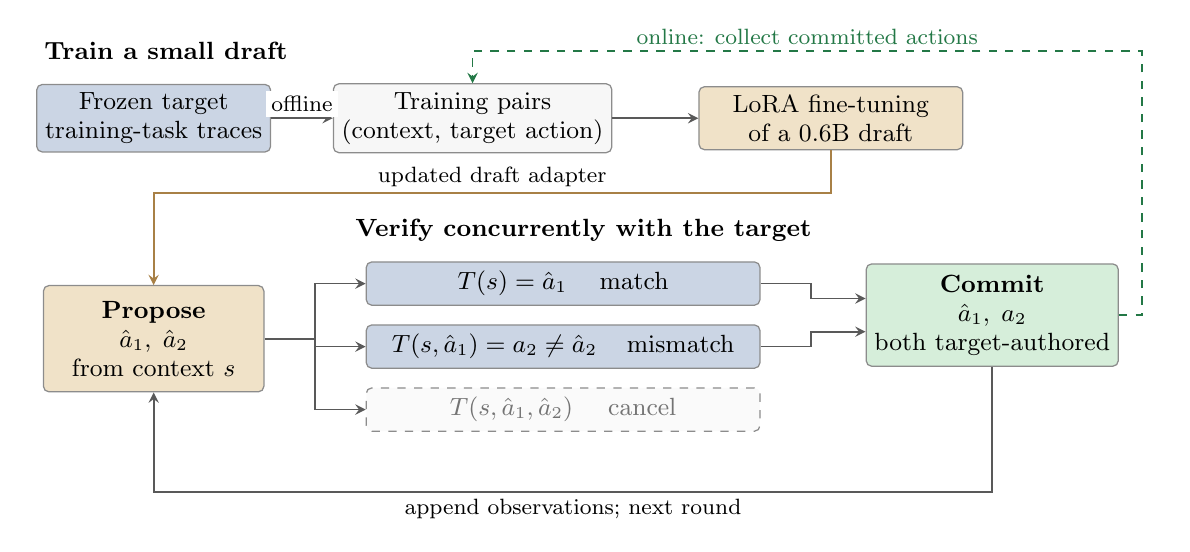
\begin{tikzpicture}[x=1cm,y=1cm,>=stealth,
 every node/.style={font=\fontsize{9}{10.5}\selectfont,inner sep=3pt},
 box/.style={draw=black!45,rounded corners=2pt,align=center,line width=.45pt},
 arr/.style={->,draw=black!65,line width=.65pt},
 tag/.style={font=\fontsize{8.5}{10}\selectfont,fill=white,inner sep=2pt}]
\useasboundingbox (-.1,.25) rectangle (14.3,6.55);
\node[anchor=west,font=\fontsize{9.5}{11}\selectfont\bfseries] at (0,6.25) {Train a small draft};
\node[box,fill=genfill,minimum width=2.8cm,minimum height=.8cm] (traces) at (1.5,5.4)
 {Frozen target\\training-task traces};
\node[box,fill=black!3,minimum width=3.25cm,minimum height=.8cm] (pairs) at (5.55,5.4)
 {Training pairs\\(context, target action)};
\node[box,fill=draftfill,minimum width=3.35cm,minimum height=.8cm] (train) at (10.1,5.4)
 {LoRA fine-tuning\\of a 0.6B draft};
\draw[arr] (traces) -- node[tag,above]{offline} (pairs);
\draw[arr] (pairs) -- (train);
\draw[arr,draw=draftline] (train.south) -- (10.1,4.45) -- node[tag,above]{updated draft adapter} (1.5,4.45) -- (1.5,3.28);
\node[anchor=west,font=\fontsize{9.5}{11}\selectfont\bfseries] at (3.95,3.98) {Verify concurrently with the target};
\node[box,fill=draftfill,minimum width=2.8cm,minimum height=1.35cm] (draft) at (1.5,2.6)
 {\textbf{Propose}\\$\hat a_1,\;\hat a_2$\\from context $s$};
\node[box,fill=genfill,minimum width=5.0cm,minimum height=.55cm] (v1) at (6.7,3.3)
 {$T(s)=\hat a_1$ \hspace{.6em} match};
\node[box,fill=genfill,minimum width=5.0cm,minimum height=.55cm] (v2) at (6.7,2.5)
 {$T(s,\hat a_1)=a_2\ne\hat a_2$ \hspace{.5em} mismatch};
\node[box,dashed,fill=black!2,text=black!55,minimum width=5.0cm,minimum height=.55cm] (v3) at (6.7,1.7)
 {$T(s,\hat a_1,\hat a_2)$ \hspace{.7em} cancel};
\draw[arr] (draft.east) -- (3.55,2.6) |- (v1.west);
\draw[arr] (3.55,2.6) |- (v2.west);
\draw[arr] (3.55,2.6) |- (v3.west);
\node[box,fill=savedfill,minimum width=3.15cm,minimum height=1.3cm] (commit) at (12.15,2.9)
 {\textbf{Commit}\\$\hat a_1,\;a_2$\\both target-authored};
\draw[arr] (v1.east) -- (9.85,3.3) |- ([yshift=6pt]commit.west);
\draw[arr] (v2.east) -- (9.85,2.5) |- ([yshift=-6pt]commit.west);
\draw[arr] (commit.south) -- (12.15,.65) -- node[tag,below]{append observations; next round} (1.5,.65) -- (draft.south);
\draw[arr,draw=savedline,dashed] (commit.east) -- (14.05,2.9) -- (14.05,6.25) --
 node[tag,above,text=savedline]{online: collect committed actions} (5.55,6.25) -- (pairs.north);
\end{tikzpicture}
\end{document}
